
 \cajita{%
Desigualdad según el coeficiente de Gini}%
{%
 \textollamada{El coeficiente de Gini permite cuantificar la distancia de la distribución a la perfecta igualdad. Su valor varía entre 0 y 1, mientras más cerca se encuentre el valor del 1, mayor será la desigualdad.} Según los resultados de la Encovi, para el año 2000 el coeficiente de Gini era 0.60. Entre 2006 y 2011, la desigualdad aumentó ligeramente de 0.56 a 0.57, respectivamente, mientras que de 2011 a 2014, se observó una reducción de la desigualdad a 0.53, por debajo de lo observado para el año 2006.}%
{%
 Coeficiente de Gini nacional} %
{%
 República de Guatemala, serie histórica por Encovi, adimensional} %
{%
 \begin{tikzpicture}[x=1pt,y=1pt]  % Created by tikzDevice version 0.7.0 on 2015-11-27 11:21:46
% !TEX encoding = UTF-8 Unicode
\definecolor[named]{fillColor}{rgb}{1.00,1.00,1.00}
\path[use as bounding box,fill=fillColor,fill opacity=0.00] (0,0) rectangle (289.08,198.74);
\begin{scope}
\path[clip] (  0.00,  0.00) rectangle (289.08,198.74);

\path[] (  0.00,  0.00) rectangle (289.08,198.74);
\end{scope}
\begin{scope}
\path[clip] (  0.00,  0.00) rectangle (289.08,198.74);

\path[] ( 12.44, 17.78) rectangle (280.54,191.48);

\path[] ( 12.44, 41.46) --
	(280.54, 41.46);

\path[] ( 12.44, 73.05) --
	(280.54, 73.05);

\path[] ( 12.44,104.63) --
	(280.54,104.63);

\path[] ( 12.44,136.21) --
	(280.54,136.21);

\path[] ( 12.44,167.80) --
	(280.54,167.80);

\path[] ( 12.44, 25.67) --
	(280.54, 25.67);

\path[] ( 12.44, 57.25) --
	(280.54, 57.25);

\path[] ( 12.44, 88.84) --
	(280.54, 88.84);

\path[] ( 12.44,120.42) --
	(280.54,120.42);

\path[] ( 12.44,152.00) --
	(280.54,152.00);

\path[] ( 12.44,183.59) --
	(280.54,183.59);

\path[] ( 50.74, 17.78) --
	( 50.74,191.48);

\path[] (114.57, 17.78) --
	(114.57,191.48);

\path[] (178.41, 17.78) --
	(178.41,191.48);

\path[] (242.24, 17.78) --
	(242.24,191.48);
\definecolor[named]{drawColor}{rgb}{0.00,0.00,1.00}

\path[draw=drawColor,line width= 1.7pt,line join=round] ( 50.74,152.94) --
	(114.57,138.59) --
	(178.41,140.92) --
	(242.24,130.29);
\definecolor[named]{drawColor}{rgb}{0.00,0.00,0.00}

\node[text=drawColor,anchor=base,inner sep=0pt, outer sep=0pt, scale=  1.01] at ( 50.74,156.90) {0.60};

\node[text=drawColor,anchor=base,inner sep=0pt, outer sep=0pt, scale=  1.01] at (114.57,126.72) {0.56};

\node[text=drawColor,anchor=base,inner sep=0pt, outer sep=0pt, scale=  1.01] at (178.41,144.88) {0.56};

\node[text=drawColor,anchor=base,inner sep=0pt, outer sep=0pt, scale=  1.01] at (242.24,118.42) {0.53};
\definecolor[named]{fillColor}{rgb}{0.00,0.00,0.00}

\path[draw=drawColor,line width= 0.1pt,line join=round,fill=fillColor] ( 12.44, 25.67) -- (280.54, 25.67);

\path[] ( 12.44, 17.78) rectangle (280.54,191.48);
\end{scope}
\begin{scope}
\path[clip] (  0.00,  0.00) rectangle (289.08,198.74);

\path[] ( 12.44, 17.78) --
	( 12.44,191.48);
\end{scope}
\begin{scope}
\path[clip] (  0.00,  0.00) rectangle (289.08,198.74);
\definecolor[named]{drawColor}{rgb}{1.00,1.00,1.00}

\node[text=drawColor,text opacity=0.00,anchor=base east,inner sep=0pt, outer sep=0pt, scale=  1.00] at (  5.32, 21.76) {0.2};

\node[text=drawColor,text opacity=0.00,anchor=base east,inner sep=0pt, outer sep=0pt, scale=  1.00] at (  5.32, 53.35) {0.3};

\node[text=drawColor,text opacity=0.00,anchor=base east,inner sep=0pt, outer sep=0pt, scale=  1.00] at (  5.32, 84.93) {0.4};

\node[text=drawColor,text opacity=0.00,anchor=base east,inner sep=0pt, outer sep=0pt, scale=  1.00] at (  5.32,116.51) {0.5};

\node[text=drawColor,text opacity=0.00,anchor=base east,inner sep=0pt, outer sep=0pt, scale=  1.00] at (  5.32,148.10) {0.6};

\node[text=drawColor,text opacity=0.00,anchor=base east,inner sep=0pt, outer sep=0pt, scale=  1.00] at (  5.32,179.68) {0.7};
\end{scope}
\begin{scope}
\path[clip] (  0.00,  0.00) rectangle (289.08,198.74);

\path[] (  8.17, 25.67) --
	( 12.44, 25.67);

\path[] (  8.17, 57.25) --
	( 12.44, 57.25);

\path[] (  8.17, 88.84) --
	( 12.44, 88.84);

\path[] (  8.17,120.42) --
	( 12.44,120.42);

\path[] (  8.17,152.00) --
	( 12.44,152.00);

\path[] (  8.17,183.59) --
	( 12.44,183.59);
\end{scope}
\begin{scope}
\path[clip] (  0.00,  0.00) rectangle (289.08,198.74);

\path[] ( 12.44, 17.78) --
	(280.54, 17.78);
\end{scope}
\begin{scope}
\path[clip] (  0.00,  0.00) rectangle (289.08,198.74);

\path[] ( 50.74, 13.51) --
	( 50.74, 17.78);

\path[] (114.57, 13.51) --
	(114.57, 17.78);

\path[] (178.41, 13.51) --
	(178.41, 17.78);

\path[] (242.24, 13.51) --
	(242.24, 17.78);
\end{scope}
\begin{scope}
\path[clip] (  0.00,  0.00) rectangle (289.08,198.74);
\definecolor[named]{drawColor}{rgb}{0.00,0.00,0.00}

\node[text=drawColor,anchor=base,inner sep=0pt, outer sep=0pt, scale=  1.00] at ( 50.74,  2.85) {2000};

\node[text=drawColor,anchor=base,inner sep=0pt, outer sep=0pt, scale=  1.00] at (114.57,  2.85) {2006};

\node[text=drawColor,anchor=base,inner sep=0pt, outer sep=0pt, scale=  1.00] at (178.41,  2.85) {2011};

\node[text=drawColor,anchor=base,inner sep=0pt, outer sep=0pt, scale=  1.00] at (242.24,  2.85) {2014};
\end{scope}
  \end{tikzpicture}}%
{%
 Instituto Nacional de Estadística} %
 
 \cajita{%
Desigualdad según el índice de Atkinson con $\varepsilon=1$}%
{%
 \textollamada{El índice de Atkinson mide la desigualdad en términos de la pérdida de bienestar social, debido a la dispersión de los ingresos, donde $\varepsilon$ se interpreta como un parámetro de aversión a la desigualdad.} Para el año 2000, el índice de Atkinson con el parámetro de aversión a la desigualdad igual a uno, era de 0.52. Al comparar entre 2006 y 2014, se observa una pequeña reducción en el índice de 0.45 a 0.41, respectivamente.}%
{%
 Índice de Atkinson nacional, con $\varepsilon=1$} %
{%
 República de Guatemala, serie histórica por Encovi, adimensional} %
{%
 \begin{tikzpicture}[x=1pt,y=1pt]  % Created by tikzDevice version 0.7.0 on 2015-11-24 06:39:09
% !TEX encoding = UTF-8 Unicode
\definecolor[named]{fillColor}{rgb}{1.00,1.00,1.00}
\path[use as bounding box,fill=fillColor,fill opacity=0.00] (0,0) rectangle (289.08,198.74);
\begin{scope}
\path[clip] (  0.00,  0.00) rectangle (289.08,198.74);

\path[] (  0.00,  0.00) rectangle (289.08,198.74);
\end{scope}
\begin{scope}
\path[clip] (  0.00,  0.00) rectangle (289.08,198.74);

\path[] ( 16.82, 17.78) rectangle (280.54,191.48);

\path[] ( 16.82, 27.01) --
	(280.54, 27.01);

\path[] ( 16.82, 70.85) --
	(280.54, 70.85);

\path[] ( 16.82,114.68) --
	(280.54,114.68);

\path[] ( 16.82,158.52) --
	(280.54,158.52);

\path[] ( 16.82, 48.93) --
	(280.54, 48.93);

\path[] ( 16.82, 92.77) --
	(280.54, 92.77);

\path[] ( 16.82,136.60) --
	(280.54,136.60);

\path[] ( 16.82,180.44) --
	(280.54,180.44);

\path[] ( 54.49, 17.78) --
	( 54.49,191.48);

\path[] (117.28, 17.78) --
	(117.28,191.48);

\path[] (180.08, 17.78) --
	(180.08,191.48);

\path[] (242.87, 17.78) --
	(242.87,191.48);
\definecolor[named]{drawColor}{rgb}{0.00,0.00,1.00}

\path[draw=drawColor,line width= 1.7pt,line join=round] ( 54.49,183.59) --
	(117.28, 99.88) --
	(180.08,103.93) --
	(242.87, 62.11);
\definecolor[named]{drawColor}{rgb}{0.00,0.00,0.00}

\node[text=drawColor,anchor=base,inner sep=0pt, outer sep=0pt, scale=  1.01] at ( 54.49,187.54) {0.52};

\node[text=drawColor,anchor=base,inner sep=0pt, outer sep=0pt, scale=  1.01] at (117.28, 88.01) {0.45};

\node[text=drawColor,anchor=base,inner sep=0pt, outer sep=0pt, scale=  1.01] at (180.08,107.89) {0.45};

\node[text=drawColor,anchor=base,inner sep=0pt, outer sep=0pt, scale=  1.01] at (242.87, 50.24) {0.41};
\definecolor[named]{fillColor}{rgb}{0.00,0.00,0.00}

\path[draw=drawColor,line width= 0.1pt,line join=round,fill=fillColor] ( 16.82, 25.67) -- (280.54, 25.67);

\path[] ( 16.82, 17.78) rectangle (280.54,191.48);
\end{scope}
\begin{scope}
\path[clip] (  0.00,  0.00) rectangle (289.08,198.74);

\path[] ( 16.82, 17.78) --
	( 16.82,191.48);
\end{scope}
\begin{scope}
\path[clip] (  0.00,  0.00) rectangle (289.08,198.74);
\definecolor[named]{drawColor}{rgb}{1.00,1.00,1.00}

\node[text=drawColor,text opacity=0.00,anchor=base east,inner sep=0pt, outer sep=0pt, scale=  1.00] at (  9.70, 45.02) {0.40};

\node[text=drawColor,text opacity=0.00,anchor=base east,inner sep=0pt, outer sep=0pt, scale=  1.00] at (  9.70, 88.86) {0.44};

\node[text=drawColor,text opacity=0.00,anchor=base east,inner sep=0pt, outer sep=0pt, scale=  1.00] at (  9.70,132.69) {0.48};

\node[text=drawColor,text opacity=0.00,anchor=base east,inner sep=0pt, outer sep=0pt, scale=  1.00] at (  9.70,176.53) {0.52};
\end{scope}
\begin{scope}
\path[clip] (  0.00,  0.00) rectangle (289.08,198.74);

\path[] ( 12.55, 48.93) --
	( 16.82, 48.93);

\path[] ( 12.55, 92.77) --
	( 16.82, 92.77);

\path[] ( 12.55,136.60) --
	( 16.82,136.60);

\path[] ( 12.55,180.44) --
	( 16.82,180.44);
\end{scope}
\begin{scope}
\path[clip] (  0.00,  0.00) rectangle (289.08,198.74);

\path[] ( 16.82, 17.78) --
	(280.54, 17.78);
\end{scope}
\begin{scope}
\path[clip] (  0.00,  0.00) rectangle (289.08,198.74);

\path[] ( 54.49, 13.51) --
	( 54.49, 17.78);

\path[] (117.28, 13.51) --
	(117.28, 17.78);

\path[] (180.08, 13.51) --
	(180.08, 17.78);

\path[] (242.87, 13.51) --
	(242.87, 17.78);
\end{scope}
\begin{scope}
\path[clip] (  0.00,  0.00) rectangle (289.08,198.74);
\definecolor[named]{drawColor}{rgb}{0.00,0.00,0.00}

\node[text=drawColor,anchor=base,inner sep=0pt, outer sep=0pt, scale=  1.00] at ( 54.49,  2.85) {2000};

\node[text=drawColor,anchor=base,inner sep=0pt, outer sep=0pt, scale=  1.00] at (117.28,  2.85) {2006};

\node[text=drawColor,anchor=base,inner sep=0pt, outer sep=0pt, scale=  1.00] at (180.08,  2.85) {2011};

\node[text=drawColor,anchor=base,inner sep=0pt, outer sep=0pt, scale=  1.00] at (242.87,  2.85) {2014};
\end{scope}
  \end{tikzpicture}}%
{%
 Instituto Nacional de Estadística} %
 
 \cajita{%
Desigualdad según el índice de Atkinson con $\varepsilon=2$}%
{%
 Cuando $\varepsilon = \mbox{2}$, el parámetro de aversión a la desigualdad aumenta y se otorga mayor peso al extremo inferior de la distribución\footnote{El índice de Atkinson con $\varepsilon = \mbox{2} $ se calcula con la fórmula: 
	\[ A = 1 - \frac{N}{\mu}\left( \sum_{i=1}^{N}\frac{1}{x_i} \right)^{-1} \]}. \\\\ Entre 2006 y 2011, el índice de Atkinson aumentó de 0.72 a 0.77, respectivamente, y de 2011 a 2014, se redujo a 0.71.  
}%
{%
 Índice de Atkinson nacional, con $\varepsilon=2$} %
{%
 República de Guatemala, serie histórica por Encovi, adimensional} %
{%
 \begin{tikzpicture}[x=1pt,y=1pt]  % Created by tikzDevice version 0.7.0 on 2015-11-27 11:35:14
% !TEX encoding = UTF-8 Unicode
\definecolor[named]{fillColor}{rgb}{1.00,1.00,1.00}
\path[use as bounding box,fill=fillColor,fill opacity=0.00] (0,0) rectangle (289.08,198.74);
\begin{scope}
\path[clip] (  0.00,  0.00) rectangle (289.08,198.74);

\path[] (  0.00,  0.00) rectangle (289.08,198.74);
\end{scope}
\begin{scope}
\path[clip] (  0.00,  0.00) rectangle (289.08,198.74);

\path[] ( 12.44, 17.78) rectangle (280.54,191.48);

\path[] ( 12.44, 65.15) --
	(280.54, 65.15);

\path[] ( 12.44,117.79) --
	(280.54,117.79);

\path[] ( 12.44,170.43) --
	(280.54,170.43);

\path[] ( 12.44, 38.83) --
	(280.54, 38.83);

\path[] ( 12.44, 91.47) --
	(280.54, 91.47);

\path[] ( 12.44,144.11) --
	(280.54,144.11);

\path[] ( 50.74, 17.78) --
	( 50.74,191.48);

\path[] (114.57, 17.78) --
	(114.57,191.48);

\path[] (178.41, 17.78) --
	(178.41,191.48);

\path[] (242.24, 17.78) --
	(242.24,191.48);
\definecolor[named]{drawColor}{rgb}{0.00,0.00,1.00}

\path[draw=drawColor,line width= 1.7pt,line join=round] ( 50.74,167.92) --
	(114.57,123.44) --
	(178.41,135.13) --
	(242.24,121.56);
\definecolor[named]{drawColor}{rgb}{0.00,0.00,0.00}

\node[text=drawColor,anchor=base,inner sep=0pt, outer sep=0pt, scale=  1.01] at ( 50.74,171.87) {0.89};

\node[text=drawColor,anchor=base,inner sep=0pt, outer sep=0pt, scale=  1.01] at (114.57,111.57) {0.72};

\node[text=drawColor,anchor=base,inner sep=0pt, outer sep=0pt, scale=  1.01] at (178.41,139.09) {0.77};

\node[text=drawColor,anchor=base,inner sep=0pt, outer sep=0pt, scale=  1.01] at (242.24,109.69) {0.71};
\definecolor[named]{fillColor}{rgb}{0.00,0.00,0.00}

\path[draw=drawColor,line width= 0.1pt,line join=round,fill=fillColor] ( 12.44, 25.67) -- (280.54, 25.67);

\path[] ( 12.44, 17.78) rectangle (280.54,191.48);
\end{scope}
\begin{scope}
\path[clip] (  0.00,  0.00) rectangle (289.08,198.74);

\path[] ( 12.44, 17.78) --
	( 12.44,191.48);
\end{scope}
\begin{scope}
\path[clip] (  0.00,  0.00) rectangle (289.08,198.74);
\definecolor[named]{drawColor}{rgb}{1.00,1.00,1.00}

\node[text=drawColor,text opacity=0.00,anchor=base east,inner sep=0pt, outer sep=0pt, scale=  1.00] at (  5.32, 34.92) {0.4};

\node[text=drawColor,text opacity=0.00,anchor=base east,inner sep=0pt, outer sep=0pt, scale=  1.00] at (  5.32, 87.56) {0.6};

\node[text=drawColor,text opacity=0.00,anchor=base east,inner sep=0pt, outer sep=0pt, scale=  1.00] at (  5.32,140.20) {0.8};
\end{scope}
\begin{scope}
\path[clip] (  0.00,  0.00) rectangle (289.08,198.74);

\path[] (  8.17, 38.83) --
	( 12.44, 38.83);

\path[] (  8.17, 91.47) --
	( 12.44, 91.47);

\path[] (  8.17,144.11) --
	( 12.44,144.11);
\end{scope}
\begin{scope}
\path[clip] (  0.00,  0.00) rectangle (289.08,198.74);

\path[] ( 12.44, 17.78) --
	(280.54, 17.78);
\end{scope}
\begin{scope}
\path[clip] (  0.00,  0.00) rectangle (289.08,198.74);

\path[] ( 50.74, 13.51) --
	( 50.74, 17.78);

\path[] (114.57, 13.51) --
	(114.57, 17.78);

\path[] (178.41, 13.51) --
	(178.41, 17.78);

\path[] (242.24, 13.51) --
	(242.24, 17.78);
\end{scope}
\begin{scope}
\path[clip] (  0.00,  0.00) rectangle (289.08,198.74);
\definecolor[named]{drawColor}{rgb}{0.00,0.00,0.00}

\node[text=drawColor,anchor=base,inner sep=0pt, outer sep=0pt, scale=  1.00] at ( 50.74,  2.85) {2000};

\node[text=drawColor,anchor=base,inner sep=0pt, outer sep=0pt, scale=  1.00] at (114.57,  2.85) {2006};

\node[text=drawColor,anchor=base,inner sep=0pt, outer sep=0pt, scale=  1.00] at (178.41,  2.85) {2011};

\node[text=drawColor,anchor=base,inner sep=0pt, outer sep=0pt, scale=  1.00] at (242.24,  2.85) {2014};
\end{scope}
  \end{tikzpicture}}%
{%
 Instituto Nacional de Estadística} %
 
 \cajita{%
Desigualdad según el índice de Theil}%
{%
   Según lo observado con las estimaciones de los índices de desigualdad anteriores, entre 2006 y 2011 hubo  un aumento de la desigualdad .\\ \\ 
 Esto es consistente con los resultados obtenidos del índice de Theil\footnote{El índice de Theil es una medida de desigualdad que está basado en la teroía de la entropía de Shannon; entre mayor sea el valor, mayor es la desigualdad. \\\\ Se calcula con la fórmula: \[ T =\frac{1}{N} \sum_{i=1}^{N}\frac{x_i}{\mu}\Logos\mbox{ln} \left(\frac{x_i}{\mu}\right) \]}, que muestran un aumento de la desigualdad en ese período. Asimismo, para el 2014, se obtiene una reducción de la desigualdad de 0.73 en 2011 a 0.60 en 2014.}%
{%
 Índice de Theil nacional} %
{%
 República de Guatemala, serie histórica por Encovi, adimensional} %
{%
 \begin{tikzpicture}[x=1pt,y=1pt]  % Created by tikzDevice version 0.7.0 on 2015-11-27 11:39:26
% !TEX encoding = UTF-8 Unicode
\definecolor[named]{fillColor}{rgb}{1.00,1.00,1.00}
\path[use as bounding box,fill=fillColor,fill opacity=0.00] (0,0) rectangle (289.08,198.74);
\begin{scope}
\path[clip] (  0.00,  0.00) rectangle (289.08,198.74);

\path[] (  0.00,  0.00) rectangle (289.08,198.74);
\end{scope}
\begin{scope}
\path[clip] (  0.00,  0.00) rectangle (289.08,198.74);

\path[] ( 12.44, 17.78) rectangle (280.54,191.48);

\path[] ( 12.44, 41.46) --
	(280.54, 41.46);

\path[] ( 12.44, 73.05) --
	(280.54, 73.05);

\path[] ( 12.44,104.63) --
	(280.54,104.63);

\path[] ( 12.44,136.21) --
	(280.54,136.21);

\path[] ( 12.44,167.80) --
	(280.54,167.80);

\path[] ( 12.44, 25.67) --
	(280.54, 25.67);

\path[] ( 12.44, 57.25) --
	(280.54, 57.25);

\path[] ( 12.44, 88.84) --
	(280.54, 88.84);

\path[] ( 12.44,120.42) --
	(280.54,120.42);

\path[] ( 12.44,152.00) --
	(280.54,152.00);

\path[] ( 12.44,183.59) --
	(280.54,183.59);

\path[] ( 50.74, 17.78) --
	( 50.74,191.48);

\path[] (114.57, 17.78) --
	(114.57,191.48);

\path[] (178.41, 17.78) --
	(178.41,191.48);

\path[] (242.24, 17.78) --
	(242.24,191.48);
\definecolor[named]{drawColor}{rgb}{0.00,0.00,1.00}

\path[draw=drawColor,line width= 1.7pt,line join=round] ( 50.74,172.06) --
	(114.57,127.71) --
	(178.41,161.21) --
	(242.24,118.98);
\definecolor[named]{drawColor}{rgb}{0.00,0.00,0.00}

\node[text=drawColor,anchor=base,inner sep=0pt, outer sep=0pt, scale=  1.01] at ( 50.74,176.01) {0.76};

\node[text=drawColor,anchor=base,inner sep=0pt, outer sep=0pt, scale=  1.01] at (114.57,115.84) {0.62};

\node[text=drawColor,anchor=base,inner sep=0pt, outer sep=0pt, scale=  1.01] at (178.41,165.17) {0.73};

\node[text=drawColor,anchor=base,inner sep=0pt, outer sep=0pt, scale=  1.01] at (242.24,107.11) {0.60};
\definecolor[named]{fillColor}{rgb}{0.00,0.00,0.00}

\path[draw=drawColor,line width= 0.1pt,line join=round,fill=fillColor] ( 12.44, 25.67) -- (280.54, 25.67);

\path[] ( 12.44, 17.78) rectangle (280.54,191.48);
\end{scope}
\begin{scope}
\path[clip] (  0.00,  0.00) rectangle (289.08,198.74);

\path[] ( 12.44, 17.78) --
	( 12.44,191.48);
\end{scope}
\begin{scope}
\path[clip] (  0.00,  0.00) rectangle (289.08,198.74);
\definecolor[named]{drawColor}{rgb}{1.00,1.00,1.00}

\node[text=drawColor,text opacity=0.00,anchor=base east,inner sep=0pt, outer sep=0pt, scale=  1.00] at (  5.32, 21.76) {0.3};

\node[text=drawColor,text opacity=0.00,anchor=base east,inner sep=0pt, outer sep=0pt, scale=  1.00] at (  5.32, 53.35) {0.4};

\node[text=drawColor,text opacity=0.00,anchor=base east,inner sep=0pt, outer sep=0pt, scale=  1.00] at (  5.32, 84.93) {0.5};

\node[text=drawColor,text opacity=0.00,anchor=base east,inner sep=0pt, outer sep=0pt, scale=  1.00] at (  5.32,116.51) {0.6};

\node[text=drawColor,text opacity=0.00,anchor=base east,inner sep=0pt, outer sep=0pt, scale=  1.00] at (  5.32,148.10) {0.7};

\node[text=drawColor,text opacity=0.00,anchor=base east,inner sep=0pt, outer sep=0pt, scale=  1.00] at (  5.32,179.68) {0.8};
\end{scope}
\begin{scope}
\path[clip] (  0.00,  0.00) rectangle (289.08,198.74);

\path[] (  8.17, 25.67) --
	( 12.44, 25.67);

\path[] (  8.17, 57.25) --
	( 12.44, 57.25);

\path[] (  8.17, 88.84) --
	( 12.44, 88.84);

\path[] (  8.17,120.42) --
	( 12.44,120.42);

\path[] (  8.17,152.00) --
	( 12.44,152.00);

\path[] (  8.17,183.59) --
	( 12.44,183.59);
\end{scope}
\begin{scope}
\path[clip] (  0.00,  0.00) rectangle (289.08,198.74);

\path[] ( 12.44, 17.78) --
	(280.54, 17.78);
\end{scope}
\begin{scope}
\path[clip] (  0.00,  0.00) rectangle (289.08,198.74);

\path[] ( 50.74, 13.51) --
	( 50.74, 17.78);

\path[] (114.57, 13.51) --
	(114.57, 17.78);

\path[] (178.41, 13.51) --
	(178.41, 17.78);

\path[] (242.24, 13.51) --
	(242.24, 17.78);
\end{scope}
\begin{scope}
\path[clip] (  0.00,  0.00) rectangle (289.08,198.74);
\definecolor[named]{drawColor}{rgb}{0.00,0.00,0.00}

\node[text=drawColor,anchor=base,inner sep=0pt, outer sep=0pt, scale=  1.00] at ( 50.74,  2.85) {2000};

\node[text=drawColor,anchor=base,inner sep=0pt, outer sep=0pt, scale=  1.00] at (114.57,  2.85) {2006};

\node[text=drawColor,anchor=base,inner sep=0pt, outer sep=0pt, scale=  1.00] at (178.41,  2.85) {2011};

\node[text=drawColor,anchor=base,inner sep=0pt, outer sep=0pt, scale=  1.00] at (242.24,  2.85) {2014};
\end{scope}
  \end{tikzpicture}}%
{%
 Instituto Nacional de Estadística} %
 
 \cajita{%
Participación del quintil más bajo}%
{%
  Para 2000, el 20\% de la población con menos recursos, captaba el 2.0\% del total de los ingresos nacionales. Al observar los resultados de las distintas Encovi, se aprecia que la participación del quintil\footnote{Un quintil es la quinta parte de una población estadística ordenada de menor a mayor en alguna característica de esta.} más bajo se ha incrementado a 3.3 \% en 2014.}%
{%
 Proporción del primer quintil de ingresos respecto del ingreso total} %
{%
 República de Guatemala, serie histórica por Encovi, en porcentaje} %
{%
 \begin{tikzpicture}[x=1pt,y=1pt]  % Created by tikzDevice version 0.9 on 2015-11-26 22:30:54
% !TEX encoding = UTF-8 Unicode
\definecolor{fillColor}{RGB}{255,255,255}
\path[use as bounding box,fill=fillColor,fill opacity=0.00] (0,0) rectangle (289.08,198.74);
\begin{scope}
\path[clip] (  0.00,  0.00) rectangle (289.08,198.74);

\path[] (  0.00,  0.00) rectangle (289.08,198.74);
\end{scope}
\begin{scope}
\path[clip] (  0.00,  0.00) rectangle (289.08,198.74);

\path[] ( 12.44, 17.78) rectangle (280.54,191.48);

\path[] ( 12.44, 41.38) --
	(280.54, 41.38);

\path[] ( 12.44, 88.16) --
	(280.54, 88.16);

\path[] ( 12.44,134.93) --
	(280.54,134.93);

\path[] ( 12.44,181.71) --
	(280.54,181.71);

\path[] ( 12.44, 18.00) --
	(280.54, 18.00);

\path[] ( 12.44, 64.77) --
	(280.54, 64.77);

\path[] ( 12.44,111.55) --
	(280.54,111.55);

\path[] ( 12.44,158.32) --
	(280.54,158.32);

\path[] ( 50.74, 17.78) --
	( 50.74,191.48);

\path[] (114.57, 17.78) --
	(114.57,191.48);

\path[] (178.41, 17.78) --
	(178.41,191.48);

\path[] (242.24, 17.78) --
	(242.24,191.48);
\definecolor{drawColor}{RGB}{0,0,255}

\path[draw=drawColor,line width= 1.7pt,line join=round] ( 50.74, 62.11) --
	(114.57,129.49) --
	(178.41,153.19) --
	(242.24,183.59);
\definecolor{drawColor}{RGB}{0,0,0}

\node[text=drawColor,anchor=base,inner sep=0pt, outer sep=0pt, scale=  1.01] at ( 50.74, 50.24) {2.0};

\node[text=drawColor,anchor=base east,inner sep=0pt, outer sep=0pt, scale=  1.01] at (112.34,129.49) {2.7};

\node[text=drawColor,anchor=base east,inner sep=0pt, outer sep=0pt, scale=  1.01] at (176.18,153.19) {2.9};

\node[text=drawColor,anchor=base,inner sep=0pt, outer sep=0pt, scale=  1.01] at (242.24,187.54) {3.3};

\path[draw=drawColor,line width= 0.1pt,line join=round] ( 12.44, 25.67) -- (280.54, 25.67);

\path[] ( 12.44, 17.78) rectangle (280.54,191.48);
\end{scope}
\begin{scope}
\path[clip] (  0.00,  0.00) rectangle (289.08,198.74);

\path[] ( 12.44, 17.78) --
	( 12.44,191.48);
\end{scope}
\begin{scope}
\path[clip] (  0.00,  0.00) rectangle (289.08,198.74);
\definecolor{drawColor}{RGB}{255,255,255}

\node[text=drawColor,text opacity=0.00,anchor=base east,inner sep=0pt, outer sep=0pt, scale=  1.00] at (  5.32, 14.09) {1.5};

\node[text=drawColor,text opacity=0.00,anchor=base east,inner sep=0pt, outer sep=0pt, scale=  1.00] at (  5.32, 60.86) {2.0};

\node[text=drawColor,text opacity=0.00,anchor=base east,inner sep=0pt, outer sep=0pt, scale=  1.00] at (  5.32,107.64) {2.5};

\node[text=drawColor,text opacity=0.00,anchor=base east,inner sep=0pt, outer sep=0pt, scale=  1.00] at (  5.32,154.41) {3.0};
\end{scope}
\begin{scope}
\path[clip] (  0.00,  0.00) rectangle (289.08,198.74);

\path[] (  8.17, 18.00) --
	( 12.44, 18.00);

\path[] (  8.17, 64.77) --
	( 12.44, 64.77);

\path[] (  8.17,111.55) --
	( 12.44,111.55);

\path[] (  8.17,158.32) --
	( 12.44,158.32);
\end{scope}
\begin{scope}
\path[clip] (  0.00,  0.00) rectangle (289.08,198.74);

\path[] ( 12.44, 17.78) --
	(280.54, 17.78);
\end{scope}
\begin{scope}
\path[clip] (  0.00,  0.00) rectangle (289.08,198.74);

\path[] ( 50.74, 13.51) --
	( 50.74, 17.78);

\path[] (114.57, 13.51) --
	(114.57, 17.78);

\path[] (178.41, 13.51) --
	(178.41, 17.78);

\path[] (242.24, 13.51) --
	(242.24, 17.78);
\end{scope}
\begin{scope}
\path[clip] (  0.00,  0.00) rectangle (289.08,198.74);
\definecolor{drawColor}{RGB}{0,0,0}

\node[text=drawColor,anchor=base,inner sep=0pt, outer sep=0pt, scale=  1.00] at ( 50.74,  2.85) {2000};

\node[text=drawColor,anchor=base,inner sep=0pt, outer sep=0pt, scale=  1.00] at (114.57,  2.85) {2006};

\node[text=drawColor,anchor=base,inner sep=0pt, outer sep=0pt, scale=  1.00] at (178.41,  2.85) {2011};

\node[text=drawColor,anchor=base,inner sep=0pt, outer sep=0pt, scale=  1.00] at (242.24,  2.85) {2014};
\end{scope}
  \end{tikzpicture}}%
{%
 Instituto Nacional de Estadística} %
 
 \cajita{%
Participación del quintil más alto}%
{%
 \textollamada{Un quintil es la quinta parte de una población estadística ordenada de menor a mayor en alguna característica de esta.} En 2014, la participación del quintil más alto era de 57.3\%, es decir, que el 20\% más rico de la población captaba más de la mitad del total de los ingresos. \\\\
Al comparar con los resultados para años anteriores, se observa que entre 2006 y 2011, hubo un aumento en la participación del quinto quintil, y de 2011 a 2014, se redujo en aproximadamente   tres puntos porcentuales.  }%
{%
 Proporción del quinto quintil de ingresos respecto del ingreso total} %
{%
 República de Guatemala, serie histórica por Encovi, en porcentaje} %
{%
 \begin{tikzpicture}[x=1pt,y=1pt]  % Created by tikzDevice version 0.7.0 on 2015-11-24 06:39:17
% !TEX encoding = UTF-8 Unicode
\definecolor[named]{fillColor}{rgb}{1.00,1.00,1.00}
\path[use as bounding box,fill=fillColor,fill opacity=0.00] (0,0) rectangle (289.08,198.74);
\begin{scope}
\path[clip] (  0.00,  0.00) rectangle (289.08,198.74);

\path[] (  0.00,  0.00) rectangle (289.08,198.74);
\end{scope}
\begin{scope}
\path[clip] (  0.00,  0.00) rectangle (289.08,198.74);

\path[] (  8.28, 17.78) rectangle (280.54,191.48);

\path[] (  8.28, 42.22) --
	(280.54, 42.22);

\path[] (  8.28, 88.73) --
	(280.54, 88.73);

\path[] (  8.28,135.23) --
	(280.54,135.23);

\path[] (  8.28,181.74) --
	(280.54,181.74);

\path[] (  8.28, 18.97) --
	(280.54, 18.97);

\path[] (  8.28, 65.48) --
	(280.54, 65.48);

\path[] (  8.28,111.98) --
	(280.54,111.98);

\path[] (  8.28,158.49) --
	(280.54,158.49);

\path[] ( 47.17, 17.78) --
	( 47.17,191.48);

\path[] (112.00, 17.78) --
	(112.00,191.48);

\path[] (176.82, 17.78) --
	(176.82,191.48);

\path[] (241.65, 17.78) --
	(241.65,191.48);
\definecolor[named]{drawColor}{rgb}{0.00,0.00,1.00}

\path[draw=drawColor,line width= 1.7pt,line join=round] ( 47.17,183.59) --
	(112.00,102.34) --
	(176.82,121.31) --
	(241.65, 62.11);
\definecolor[named]{drawColor}{rgb}{0.00,0.00,0.00}

\node[text=drawColor,anchor=base,inner sep=0pt, outer sep=0pt, scale=  1.01] at ( 47.17,187.54) {63.8};

\node[text=drawColor,anchor=base,inner sep=0pt, outer sep=0pt, scale=  1.01] at (112.00, 90.47) {59.5};

\node[text=drawColor,anchor=base,inner sep=0pt, outer sep=0pt, scale=  1.01] at (176.82,125.27) {60.5};

\node[text=drawColor,anchor=base,inner sep=0pt, outer sep=0pt, scale=  1.01] at (241.65, 50.24) {57.3};
\definecolor[named]{fillColor}{rgb}{0.00,0.00,0.00}

\path[draw=drawColor,line width= 0.1pt,line join=round,fill=fillColor] (  8.28, 25.67) -- (280.54, 25.67);

\path[] (  8.28, 17.78) rectangle (280.54,191.48);
\end{scope}
\begin{scope}
\path[clip] (  0.00,  0.00) rectangle (289.08,198.74);

\path[] (  8.28, 17.78) --
	(  8.28,191.48);
\end{scope}
\begin{scope}
\path[clip] (  0.00,  0.00) rectangle (289.08,198.74);
\definecolor[named]{drawColor}{rgb}{1.00,1.00,1.00}

\node[text=drawColor,text opacity=0.00,anchor=base east,inner sep=0pt, outer sep=0pt, scale=  1.00] at (  1.17, 15.06) {55.0};

\node[text=drawColor,text opacity=0.00,anchor=base east,inner sep=0pt, outer sep=0pt, scale=  1.00] at (  1.17, 61.57) {57.5};

\node[text=drawColor,text opacity=0.00,anchor=base east,inner sep=0pt, outer sep=0pt, scale=  1.00] at (  1.17,108.07) {60.0};

\node[text=drawColor,text opacity=0.00,anchor=base east,inner sep=0pt, outer sep=0pt, scale=  1.00] at (  1.17,154.58) {62.5};
\end{scope}
\begin{scope}
\path[clip] (  0.00,  0.00) rectangle (289.08,198.74);

\path[] (  4.01, 18.97) --
	(  8.28, 18.97);

\path[] (  4.01, 65.48) --
	(  8.28, 65.48);

\path[] (  4.01,111.98) --
	(  8.28,111.98);

\path[] (  4.01,158.49) --
	(  8.28,158.49);
\end{scope}
\begin{scope}
\path[clip] (  0.00,  0.00) rectangle (289.08,198.74);

\path[] (  8.28, 17.78) --
	(280.54, 17.78);
\end{scope}
\begin{scope}
\path[clip] (  0.00,  0.00) rectangle (289.08,198.74);

\path[] ( 47.17, 13.51) --
	( 47.17, 17.78);

\path[] (112.00, 13.51) --
	(112.00, 17.78);

\path[] (176.82, 13.51) --
	(176.82, 17.78);

\path[] (241.65, 13.51) --
	(241.65, 17.78);
\end{scope}
\begin{scope}
\path[clip] (  0.00,  0.00) rectangle (289.08,198.74);
\definecolor[named]{drawColor}{rgb}{0.00,0.00,0.00}

\node[text=drawColor,anchor=base,inner sep=0pt, outer sep=0pt, scale=  1.00] at ( 47.17,  2.85) {2000};

\node[text=drawColor,anchor=base,inner sep=0pt, outer sep=0pt, scale=  1.00] at (112.00,  2.85) {2006};

\node[text=drawColor,anchor=base,inner sep=0pt, outer sep=0pt, scale=  1.00] at (176.82,  2.85) {2011};

\node[text=drawColor,anchor=base,inner sep=0pt, outer sep=0pt, scale=  1.00] at (241.65,  2.85) {2014};
\end{scope}
  \end{tikzpicture}}%
{%
 Instituto Nacional de Estadística} %
 
 \cajita{%
Relación de ingresos del quintil más alto y más bajo}%
{%
 \textollamada[*]{La relación de ingresos del quintil más rico y el quintil más pobre se obtiene dividiendo la participación del quinto quintil  sobre la participación del primer quintil.} Para 2014, el quintil de mayores ingresos captaba 17.5 veces más que la quinta parte de la población de menos recursos.\\\\ En general, los resultados muestran una reducción en la relación de los ingresos del quintil más alto y el más bajo de 2000 a 2014. }%
{%
 Razón del quinto y primer quintil de ingresos} %
{%
 República de Guatemala, serie histórica por Encovi, adimensional} %
{%
 \begin{tikzpicture}[x=1pt,y=1pt]  % Created by tikzDevice version 0.7.0 on 2015-11-27 11:45:03
% !TEX encoding = UTF-8 Unicode
\definecolor[named]{fillColor}{rgb}{1.00,1.00,1.00}
\path[use as bounding box,fill=fillColor,fill opacity=0.00] (0,0) rectangle (289.08,198.74);
\begin{scope}
\path[clip] (  0.00,  0.00) rectangle (289.08,198.74);

\path[] (  0.00,  0.00) rectangle (289.08,198.74);
\end{scope}
\begin{scope}
\path[clip] (  0.00,  0.00) rectangle (289.08,198.74);

\path[] (  1.64, 17.78) rectangle (280.54,191.48);

\path[] (  1.64, 41.46) --
	(280.54, 41.46);

\path[] (  1.64, 73.05) --
	(280.54, 73.05);

\path[] (  1.64,104.63) --
	(280.54,104.63);

\path[] (  1.64,136.21) --
	(280.54,136.21);

\path[] (  1.64,167.80) --
	(280.54,167.80);

\path[] (  1.64, 25.67) --
	(280.54, 25.67);

\path[] (  1.64, 57.25) --
	(280.54, 57.25);

\path[] (  1.64, 88.84) --
	(280.54, 88.84);

\path[] (  1.64,120.42) --
	(280.54,120.42);

\path[] (  1.64,152.00) --
	(280.54,152.00);

\path[] (  1.64,183.59) --
	(280.54,183.59);

\path[] ( 41.49, 17.78) --
	( 41.49,191.48);

\path[] (107.89, 17.78) --
	(107.89,191.48);

\path[] (174.30, 17.78) --
	(174.30,191.48);

\path[] (240.70, 17.78) --
	(240.70,191.48);
\definecolor[named]{drawColor}{rgb}{0.00,0.00,1.00}

\path[draw=drawColor,line width= 1.7pt,line join=round] ( 41.49,167.07) --
	(107.89,102.08) --
	(174.30, 92.27) --
	(240.70, 73.23);
\definecolor[named]{drawColor}{rgb}{0.00,0.00,0.00}

\node[text=drawColor,anchor=base,inner sep=0pt, outer sep=0pt, scale=  1.01] at ( 41.49,171.02) {32.4};

\node[text=drawColor,anchor=base west,inner sep=0pt, outer sep=0pt, scale=  1.01] at (107.89,106.04) {22.1};

\node[text=drawColor,anchor=base west,inner sep=0pt, outer sep=0pt, scale=  1.01] at (174.30, 96.22) {20.5};

\node[text=drawColor,anchor=base,inner sep=0pt, outer sep=0pt, scale=  1.01] at (240.70, 61.36) {17.5};
\definecolor[named]{fillColor}{rgb}{0.00,0.00,0.00}

\path[draw=drawColor,line width= 0.1pt,line join=round,fill=fillColor] (  1.64, 25.67) -- (280.54, 25.67);

\path[] (  1.64, 17.78) rectangle (280.54,191.48);
\end{scope}
\begin{scope}
\path[clip] (  0.00,  0.00) rectangle (289.08,198.74);

\path[] (  1.64, 17.78) --
	(  1.64,191.48);
\end{scope}
\begin{scope}
\path[clip] (  0.00,  0.00) rectangle (289.08,198.74);

\path[] (  0.00, 25.67) --
	(  1.64, 25.67);

\path[] (  0.00, 57.25) --
	(  1.64, 57.25);

\path[] (  0.00, 88.84) --
	(  1.64, 88.84);

\path[] (  0.00,120.42) --
	(  1.64,120.42);

\path[] (  0.00,152.00) --
	(  1.64,152.00);

\path[] (  0.00,183.59) --
	(  1.64,183.59);
\end{scope}
\begin{scope}
\path[clip] (  0.00,  0.00) rectangle (289.08,198.74);

\path[] (  1.64, 17.78) --
	(280.54, 17.78);
\end{scope}
\begin{scope}
\path[clip] (  0.00,  0.00) rectangle (289.08,198.74);

\path[] ( 41.49, 13.51) --
	( 41.49, 17.78);

\path[] (107.89, 13.51) --
	(107.89, 17.78);

\path[] (174.30, 13.51) --
	(174.30, 17.78);

\path[] (240.70, 13.51) --
	(240.70, 17.78);
\end{scope}
\begin{scope}
\path[clip] (  0.00,  0.00) rectangle (289.08,198.74);
\definecolor[named]{drawColor}{rgb}{0.00,0.00,0.00}

\node[text=drawColor,anchor=base,inner sep=0pt, outer sep=0pt, scale=  1.00] at ( 41.49,  2.85) {2000};

\node[text=drawColor,anchor=base,inner sep=0pt, outer sep=0pt, scale=  1.00] at (107.89,  2.85) {2006};

\node[text=drawColor,anchor=base,inner sep=0pt, outer sep=0pt, scale=  1.00] at (174.30,  2.85) {2011};

\node[text=drawColor,anchor=base,inner sep=0pt, outer sep=0pt, scale=  1.00] at (240.70,  2.85) {2014};
\end{scope}
  \end{tikzpicture}}%
{%
 Instituto Nacional de Estadística} %
 
 \cajota{%
Desigualdad en los departamentos según el coeficiente de Gini }%
{%
 Al desagregar por departamento, se observa mayor desigualdad \textemdash medida por el coeficiente de Gini\footnote{El coeficiente de Gini permite cuantificar la distancia de la distribución a la perfecta igualdad. Su valor varía entre 0 y 1, mientras más cerca se encuentre el valor del 1, mayor será la desigualdad.} \textemdash en los departamentos de San Marcos (0.61), Jalapa (0.58) y Quetzaltenango (0.58). Los departamentos con menor coeficiente de Gini son Sololá (0.39),  El Progreso  (0.42) y Escuintla (0.42).}%
{%
 Coeficiente de Gini por departamento} %
{%
 Por departamento, año 2014, adimensional} %
{%
 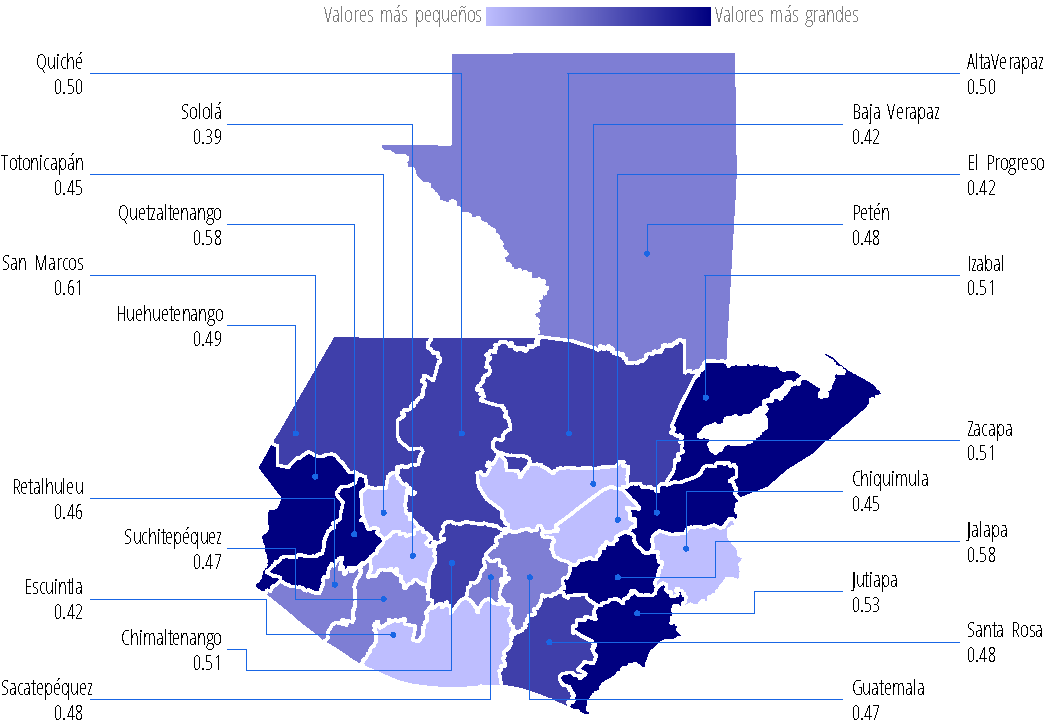
\includegraphics[width=52\cuadri]{graficas/2_08.pdf}}%
{%
 Instituto Nacional de Estadística} %
 
 \cajota{%
Desigualdad en los departamentos según el índice de Atkinson con $\varepsilon = 1$}%
{%
 Los departamentos que muestran mayor desigualdad según el índice de Atkinson\footnote{El índice de Atkinson mide la desigualdad en términos de la pérdida de bienestar social, debido a la dispersión de los ingresos, donde $\varepsilon$ se interpreta como un parámetro de aversión a la desigualdad.} (con $\varepsilon = \mbox{1}$), son San Marcos (0.52), Jalapa (0.47) y Quetzaltenago (0.46), que coinciden con los departamentos que mostraron mayor desigualdad  medida a través del coeficiente de Gini.\\\\
 Asimismo, los departamentos que muestran menor desigualdad con este índice, son Sololá, Escuintla y El progreso, con 0.24, 0.27 y 0.27, respectivamente. }%
{%
 Índice de Atkinson por departamento con $\varepsilon = 1$} %
{%
 Por departamento, año 2014, adimensional} %
{%
 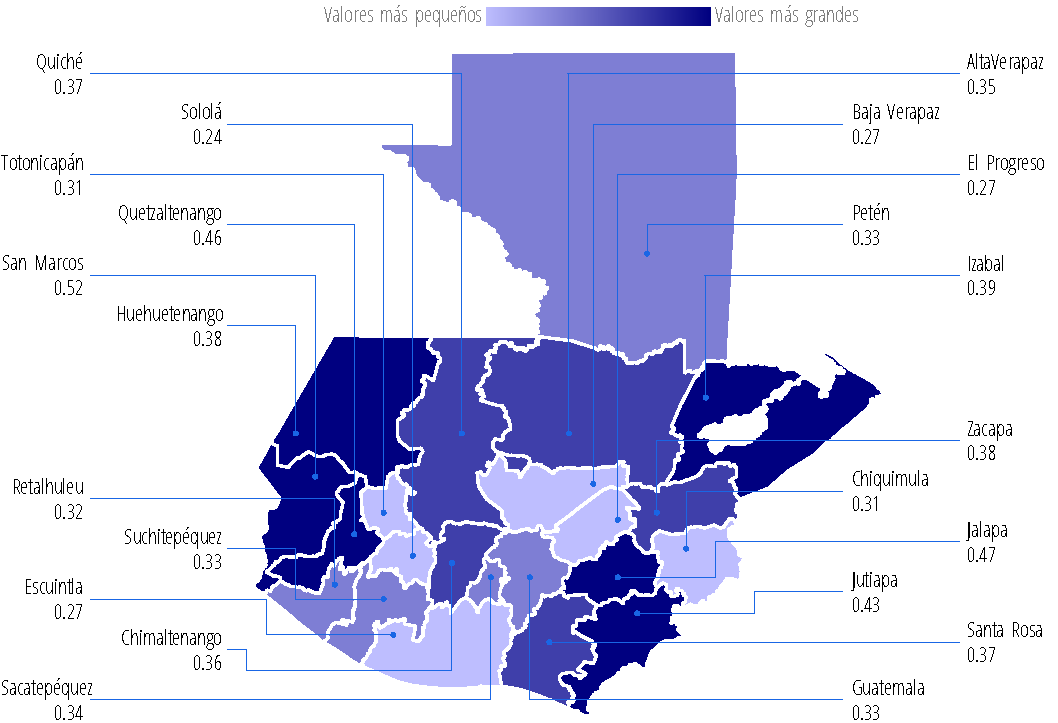
\includegraphics[width=52\cuadri]{graficas/2_09.pdf}}%
{%
 Instituto Nacional de Estadística} %
 
 \cajota{%
Desigualdad en los departamentos según el índice de Atkinson con $\varepsilon = 2$}%
{%
 Al aumentar el parámetro de aversión a la desigualdad, donde se pone mayor énfasis al extremo inferior de la distribución  ($\varepsilon = \mbox{2}$), los resultados que se venían observando se modifican. El departamento de San Marcos (0.83), sigue mostrando el mayor nivel desigualdad; no obstante, se observa cómo aumenta el índice de Atkinson para otros departamentos, como Totonicapán  que con $\varepsilon = \mbox{1}$ era uno de los menos desiguales y con $\varepsilon = \mbox{2}$ es el segundo más desigual (0.77).  \\\\ Los departamentos de Sololá (0.45), Escuintla (0.45) y El Progreso (0.48), muestran los niveles de desigualdad más bajos con el índice de Atkinson con  $\varepsilon = \mbox{2}$.}%
{%
 Índice de Atkinson por departamento con $\varepsilon = 2$} %
{%
 Por departamento, año 2014, adimensional} %
{%
 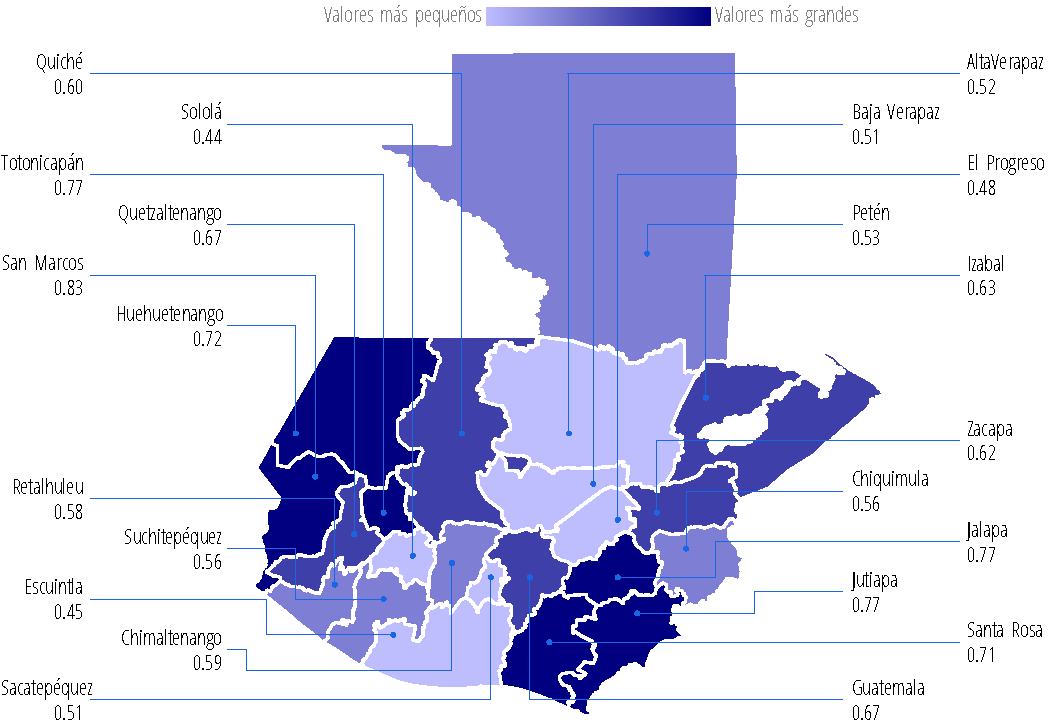
\includegraphics[width=52\cuadri]{graficas/2_10.pdf}}%
{%
 Instituto Nacional de Estadística} %
 
 \cajota{%
Desigualdad en los departamentos según el índice de Theil}%
{%
 El departamento de San Marcos (0.97) muestra el mayor nivel de desigualdad, medida a través del índice Theil\footnote{El índice de Theil es una medida de desigualdad que está basado en la entropía de Shannon; entre mayor sea el valor, mayor es la desigualdad.}, al igual que para el resto de las estimaciones anteriores;  le sigue el departamento de Quetzaltenango (0.76) y Jalapa (0.75). \\\\
 Los niveles de desigualdad más bajos, se observan en los departamentos de Baja Verapaz y El Progreso, con 0.30 ambos departamentos, y Sololá con un índice de Theil de 0.28.}%
{%
 Índice de Theil por departamento} %
{%
 Por departamento, Año 2014, adimensional} %
{%
 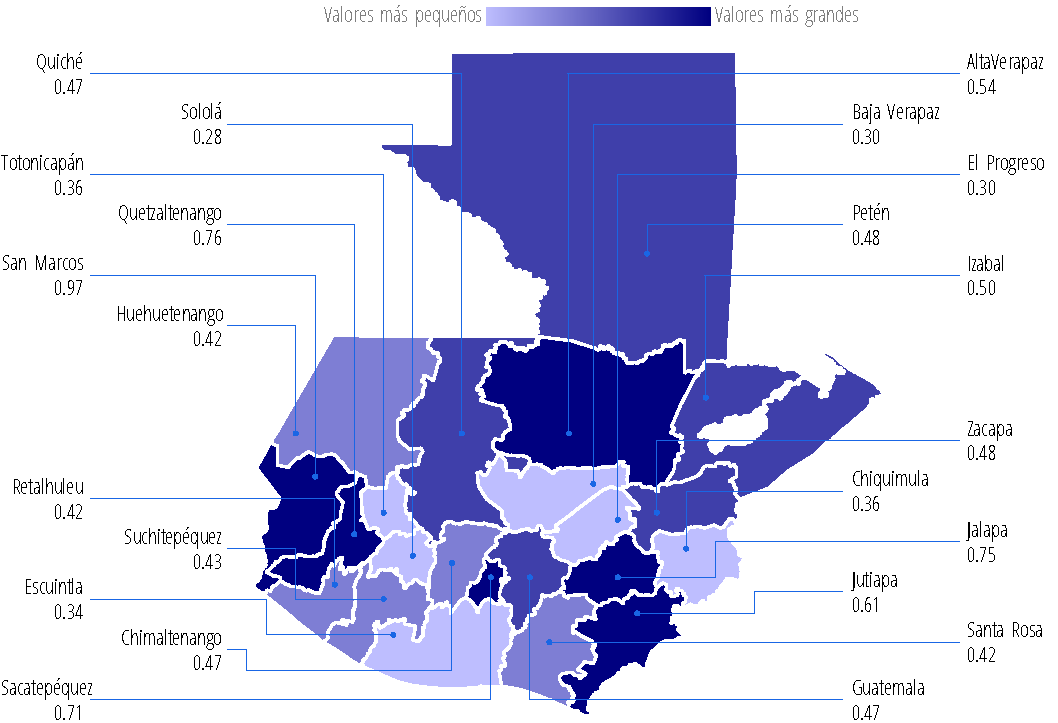
\includegraphics[width=52\cuadri]{graficas/2_11.pdf}}%
{%
 Instituto Nacional de Estadística} %
 